% ─────────────────────────────────────────────────────────────────
\section{Model Architectures}
\label{sec:arch}
% ─────────────────────────────────────────────────────────────────

\subsection{Flat GNN Baseline}
\label{sec:arch:flat}

As a baseline we train a flat single-level GNN (\texttt{classify\_gnn.py})
directly on the 1\,000-node surface graphs.
The model uses 6-layer GINs~\cite{gin} with hidden dimension 512, followed by
global sum/mean/max readout and an MLP head.
Eight backbone types (GIN, GAT, GATv2, GCN, GraphSAGE, GPS, SGFormer, PNA)
are evaluated under the same hyperparameter budget.
The best flat-GNN macro-F1 on the test set is \textbf{0.640}; it serves as
a lower baseline throughout.

\subsection{Hierarchical GNN: HierGIN}
\label{sec:arch:hier}

\begin{figure}[h]
  \centering
  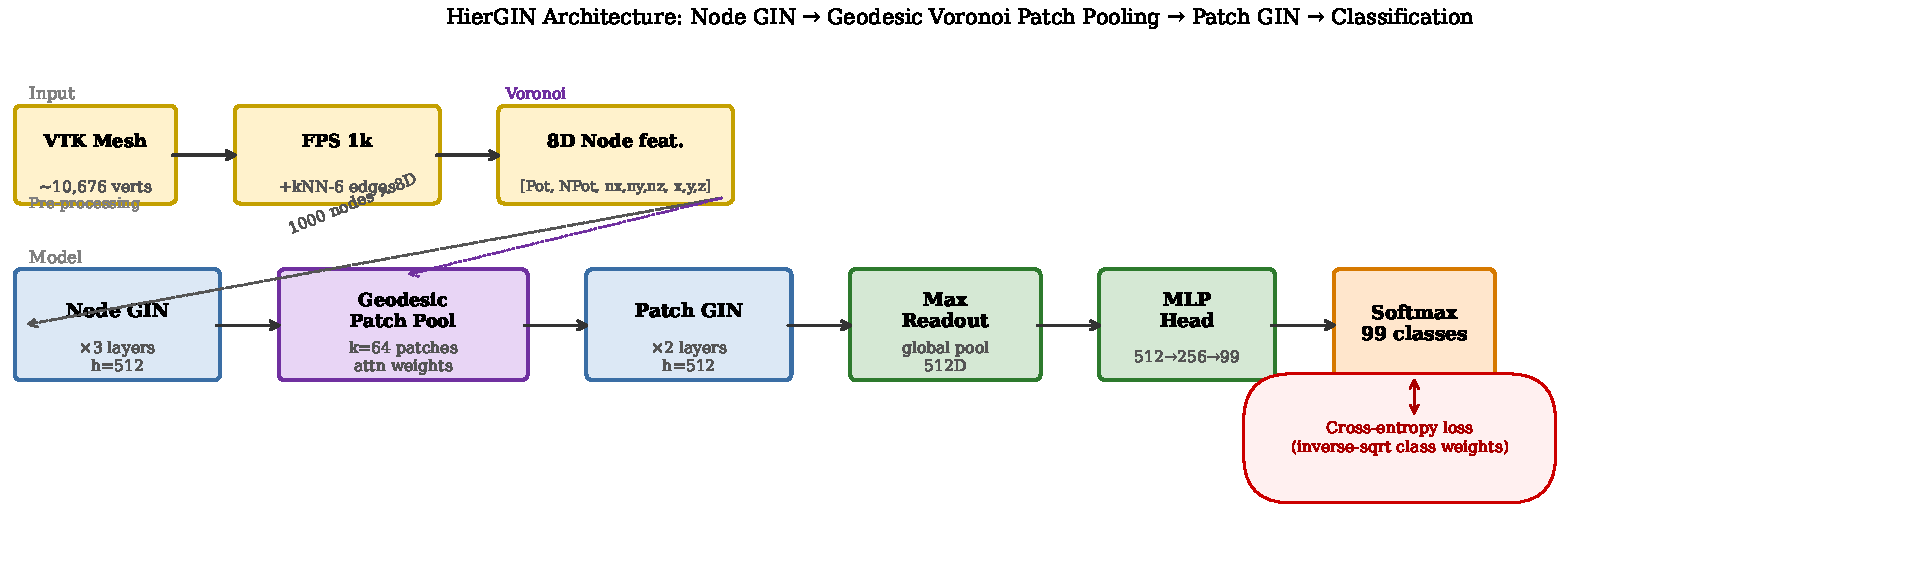
\includegraphics[width=\linewidth]{figures/architecture_diagram.pdf}
  \caption{HierGIN architecture.
           A node-level GIN processes 1\,000-node surface graphs; a geodesic
           Voronoi pooling layer coarsens to 64 patch nodes; a patch-level GIN
           refines patch representations; global max readout feeds an MLP
           classifier.}
  \label{fig:arch}
\end{figure}

The core model is a two-level hierarchical GNN
(\texttt{classify\_hierarchical\_gnn.py}) illustrated in
Figure~\ref{fig:arch}.

\subsubsection{Node-level GIN}

The first level applies $L_n = 3$ layers of a Graph Isomorphism Network
(GIN)~\cite{gin} to all 1\,000 surface nodes.
Each GIN layer applies the update:
\begin{equation}
  \mathbf{h}_i^{(\ell)} = \mathrm{MLP}\!\left(
    (1 + \epsilon)\,\mathbf{h}_i^{(\ell-1)} +
    \sum_{j \in \mathcal{N}(i)} \mathbf{h}_j^{(\ell-1)}
  \right),
  \label{eq:gin}
\end{equation}
with a 2-layer MLP per GIN layer, batch normalisation, and ReLU activation.
The initial node features $\mathbf{h}_i^{(0)} = \mathbf{x}_i \in \mathbb{R}^d$
are the raw surface features described in Section~\ref{sec:pipeline:ssl}.

In ablations we also test replacing GIN with GATv2, GAT, GraphSAGE, GCN, GPS,
SGFormer, and PNA at the node level.

\subsubsection{Geodesic Voronoi Patch Pooling}
\label{sec:arch:pool}

After node-level processing, the graph is coarsened using the geodesic Voronoi
decomposition computed in Stage~2 of the pipeline
(Section~\ref{sec:pipeline:patch}).
Each of the $k = 64$ patches aggregates its constituent node embeddings into a
single patch embedding $\mathbf{p}_c$ via attention-weighted pooling:
\begin{equation}
  \mathbf{p}_c = \sum_{i \in \mathcal{P}_c}
  \frac{\exp\!\left(\mathbf{a}^\top \mathbf{h}_i^{(L_n)}\right)}
       {\sum_{j \in \mathcal{P}_c} \exp\!\left(\mathbf{a}^\top \mathbf{h}_j^{(L_n)}\right)}
  \mathbf{h}_i^{(L_n)},
  \label{eq:attn_pool}
\end{equation}
where $\mathbf{a} \in \mathbb{R}^h$ is a learned attention vector.
We also experiment with mean pooling and max pooling over patch members, but
attention pooling achieves the highest validation F1.

\subsubsection{Patch-level GIN}

The 64 patch embeddings and the patch meta-graph (Section~\ref{sec:pipeline:patch})
are fed into $L_p = 2$ additional GIN layers with the same hidden dimension $h = 512$.
This allows patch-to-patch message passing over the coarsened surface topology,
capturing mid-scale shape features that a single-level GNN would miss.

\subsubsection{Readout and Classification}

Global max readout over all 64 patch embeddings produces a single
512-dimensional graph embedding.
A two-layer MLP (512 $\to$ 256 $\to$ 99) with dropout $p = 0.3$ between
layers maps the embedding to class logits.

\subsection{Node Backbone Variants}

Table~\ref{tab:backbones} compares all eight node backbone types under the
same hyperparameter configuration (h=512, 3 node layers, 2 patch layers,
attention patch pooling, cosine LR, 80 epochs, 4D features).

\begin{table}[h]
  \centering
  \caption{Node backbone ablation (4D features, h=512, proper eval over 88 classes).
           * PNA evaluated from training-time metrics due to inference crash
           (missing delta parameter); indicated values are slightly lower bound.}
  \label{tab:backbones}
  \begin{tabular}{lrrrr}
    \toprule
    \textbf{Backbone} & \textbf{Accuracy} & \textbf{Bal.\ Acc.} & \textbf{Macro-F1} & \textbf{Wtd-F1} \\
    \midrule
    \textbf{GIN}     & \textbf{0.8447} & \textbf{0.7955} & \textbf{0.7839} & \textbf{0.8434} \\
    GATv2            & 0.8360 & 0.7865 & 0.7741 & 0.8327 \\
    GAT              & 0.8390 & 0.7833 & 0.7739 & 0.8343 \\
    GPS              & 0.8265 & 0.7719 & 0.7615 & 0.8232 \\
    SGFormer         & 0.8295 & 0.7826 & 0.7627 & 0.8310 \\
    GCN              & 0.8291 & 0.7679 & 0.7543 & 0.8260 \\
    GraphSAGE        & 0.8230 & 0.7750 & 0.7519 & 0.8216 \\
    PNA*             & 0.7884 & 0.5640 & 0.5530 & 0.7708 \\
    \bottomrule
  \end{tabular}
\end{table}

GIN achieves the best macro-F1 ($0.784$) despite its relative simplicity.
GATv2 and GAT are competitive on accuracy but slightly worse on macro-F1.
PNA significantly underperforms, likely because its degree-based scaler
amplification is miscalibrated on the sparse 6-NN graph topology.

Figure~\ref{fig:training_curves_all} shows the validation training curves for
all eight backbones.

\begin{figure}[h]
  \centering
  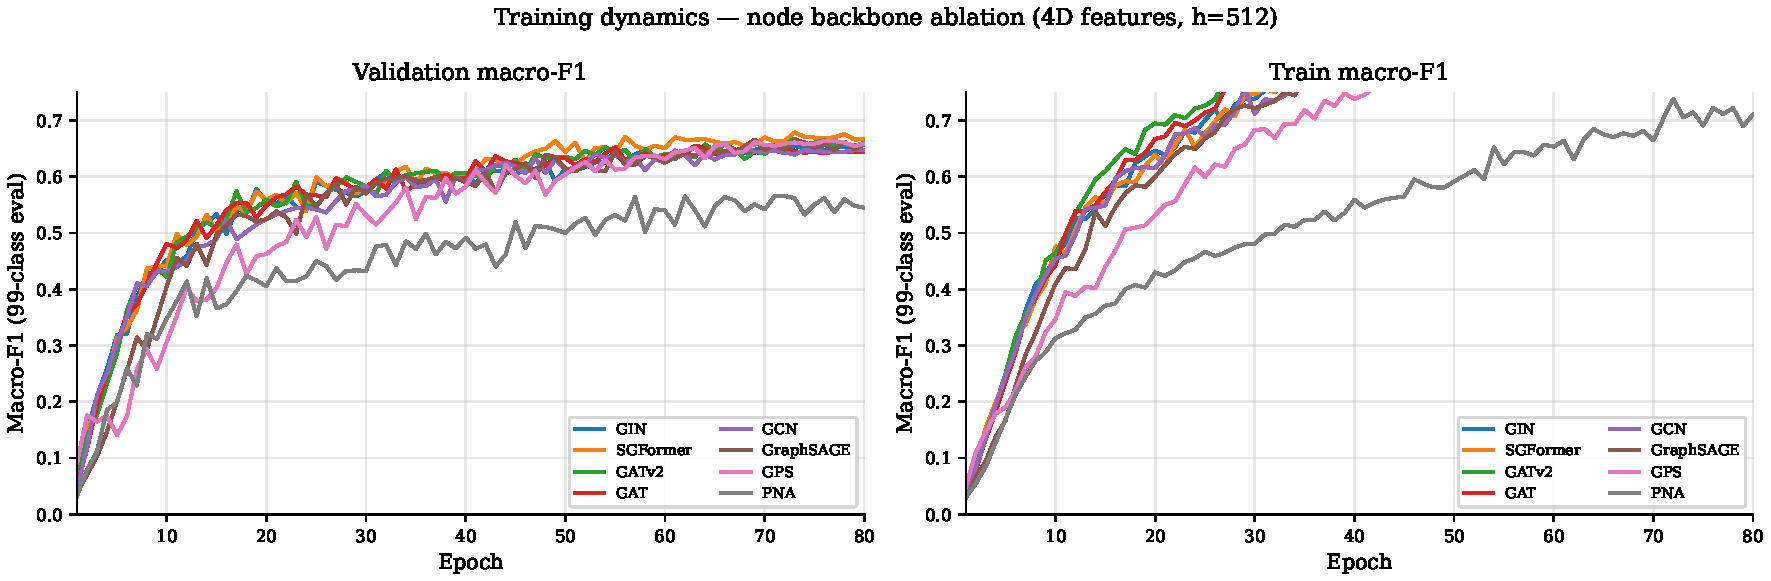
\includegraphics[width=\linewidth]{figures/training_curves_all.pdf}
  \caption{Validation macro-F1 (left) and training macro-F1 (right) over 80 epochs
           for the backbone ablation.
           All eight backbones use 4D features and are otherwise identical.}
  \label{fig:training_curves_all}
\end{figure}

\subsection{Rotation-Invariant Node Backbone: RI-GIN}
\label{sec:arch:rigin}

Standard GIN (Equation~\ref{eq:gin}) is not rotation-invariant: the node
features $\mathbf{x}_i$ include surface normals $(n_x, n_y, n_z)$ and
coordinates $(x, y, z)$ expressed in an arbitrary global frame.
Two proteins with identical surface structure but different orientations
produce different input features and therefore different embeddings.

To remove this frame dependence we implement a \textbf{rotation-invariant
node backbone} (RI-GIN), inspired by RIConv2~\cite{riconv2}.
For each directed edge $i \to j$, five SO(3)-invariant scalars are computed
on the fly from the node positions and normals:

\begin{equation}
  \mathbf{r}_{ij} = \Bigl[
    \|\mathbf{p}_j - \mathbf{p}_i\|,\;
    \langle \mathbf{n}_i,\, \hat{\mathbf{e}}_{ij} \rangle,\;
    \langle \mathbf{n}_j,\, \hat{\mathbf{e}}_{ij} \rangle,\;
    \langle \mathbf{n}_i,\, \mathbf{n}_j \rangle,\;
    \langle \mathbf{n}_j \times \mathbf{n}_i,\, \hat{\mathbf{e}}_{ij} \rangle
  \Bigr] \in \mathbb{R}^5,
  \label{eq:ri_scalars}
\end{equation}

where $\hat{\mathbf{e}}_{ij} = (\mathbf{p}_j - \mathbf{p}_i) /
\|\mathbf{p}_j - \mathbf{p}_i\|$ is the unit edge direction.
These five quantities are invariant to global rotations and reflections.
The message from node $i$ to node $j$ is then:

\begin{equation}
  \mathbf{m}_{ij} = \mathrm{MLP}_\text{edge}
    \!\left(\bigl[\mathbf{h}_i^{(\ell-1)} \;\|\; \mathbf{r}_{ij}\bigr]\right),
  \label{eq:ri_msg}
\end{equation}

and the node update aggregates incoming messages by summation:
$\mathbf{h}_i^{(\ell)} = \sum_{j \in \mathcal{N}(i)} \mathbf{m}_{ji}$,
with self-information entering through the self-loop edge (distance $\approx 0$,
$\langle \mathbf{n}_i, \mathbf{n}_i \rangle = 1$).

\paragraph{Computational note.}
Because the edge MLP operates on $[\mathbf{h}_i \,\|\, \mathbf{r}_{ij}] \in
\mathbb{R}^{h+5}$ for every edge simultaneously, it materialises dense
$[E, h]$ tensors on the GPU.
At $h = 512$ and batch size 64 (approximately 384\,000 edges), each layer
of RI-GIN creates $\sim$750\,MB of edge activations --- roughly six times
the memory footprint of standard GIN, which aggregates only $[N, h]$ node
tensors.
This constrains the practical batch size to 32 at $h = 512$ on a 12\,GB
GPU.
A memory-efficient alternative would compute RI messages at a lower
dimension (e.g.\ $d = 64$) and add them to the standard GIN update,
rather than concatenating into the full MLP.

\subsection{VTK Mesh Visualisation}

Figure~\ref{fig:vtk} shows five example protein surfaces per class for
each of the three confusable pairs, coloured by electrostatic potential.
The visual similarity between classes within each pair --- particularly
(61,\,90) --- explains the challenge of automated discrimination.

\begin{figure}[h]
  \centering
  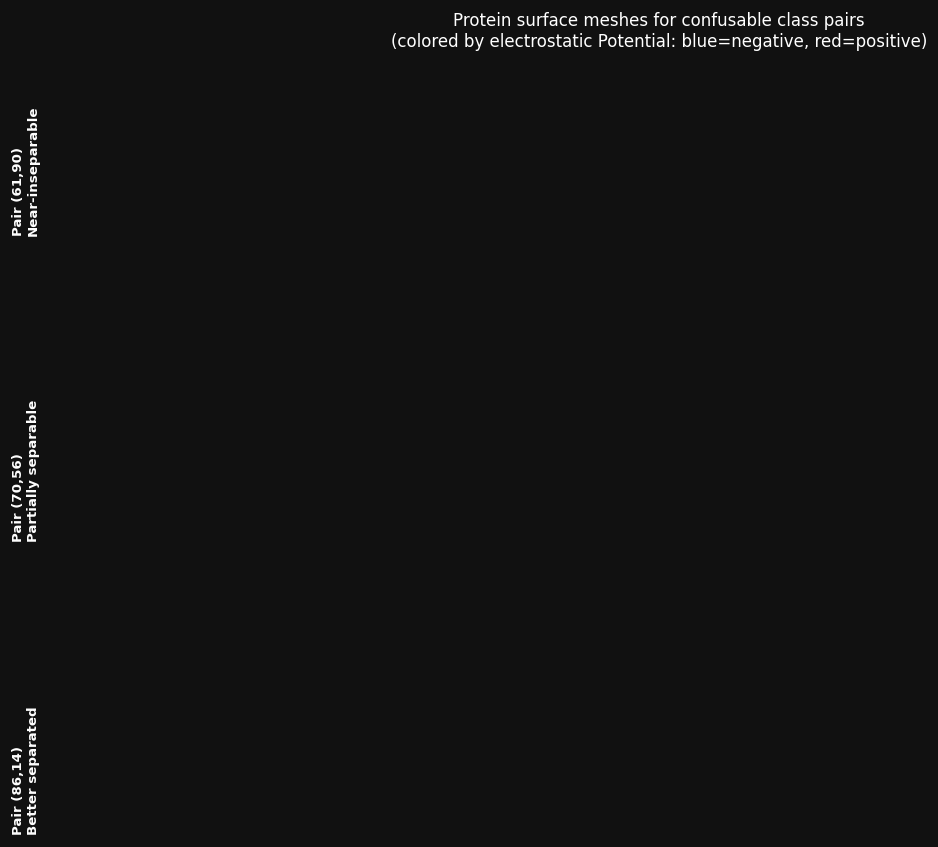
\includegraphics[width=\linewidth]{figures/vtk_mesh_showcase.png}
  \caption{Protein surface meshes for the three confusable class pairs
           (N=5 per class).
           Colour: blue = negative potential, red = positive potential.
           Classes 61 and 90 (top pair) show near-identical surface topologies
           and charge patterns, explaining their near-inseparability.}
  \label{fig:vtk}
\end{figure}
